In this section, we provide some information about the framework of meta reinforcement learning.

\par
In the framework of reinforcement learning, the agent is continuously interacting with the environment to learn an optimal strategy in order to get a maximal future reward. Such a model can be framed as a Markov Decision Process (MDP) as depicted in the following Fig. \ref{mdp}.

\begin{figure}
	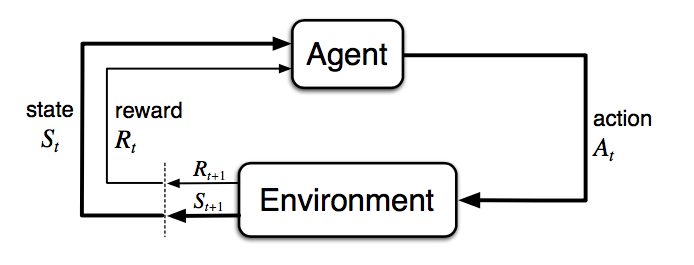
\includegraphics[scale=0.3]{mdp.png}
	\centering
	\caption{The agent-environment interaction in a Markov decision process\cite{n-step-return}.}
	\label{mdp}
\end{figure}

A Markov decision process consists of five elements $\mathcal{M} = \langle \mathcal{S}, \mathcal{A}, P, R, \gamma \rangle$, whose definition is shown in the following table:

\begin{center}
	\begin{tabular}{| p{0.12\linewidth} | p{0.27\linewidth} | p{0.45\linewidth} |}
		\hline
		\textbf{symbol} & \textbf{definition} & \textbf{function} \\
		\hline
		$\mathcal{S}$ & states of the agent &  \\ 
		\hline
		$\mathcal{A}$ & actions that the agent can choose &  \\ 
		\hline 
		$P$ & transition probability function & transition function:\newline $\mathcal{P}: \mathcal{S} \times \mathcal{A} \times \mathcal{S} \times \mathcal{R} \rightarrow \mathbb{R}_{\geq 0}$\newline state-transition function:\newline $\mathcal{P}: \mathcal{S} \times \mathcal{A} \times \mathcal{S} \rightarrow \mathbb{R}_{\geq 0}$\\
		\hline 
		$R$ & reward function & $\mathcal{R}: \mathcal{S} \times \mathcal{A} \rightarrow \mathbb{R}$ \\
		\hline 
		$\gamma$ & discounting factor for future rewards &  \\
		\hline 
	\end{tabular}
\end{center}

\par
Except for the notation of MDP, the reinforcement learning framework also consists of the following components:

\begin{center}
	\begin{tabular}{| p{0.12\linewidth} | p{0.27\linewidth} | p{0.45\linewidth} |}
		\hline
		\textbf{symbol} & \textbf{definition} & \textbf{function} \\
		\hline
		$\pi$ & policy function & deterministic:\newline $\pi: \mathcal{S} \rightarrow \mathcal{A}$ \newline stochastic:\newline $\pi: \mathcal{S} \times \mathcal{A} \rightarrow \mathbb{R}_{\geq 0}$\\ 
		\hline
		$G$ & return function & $G_{t} = \sum_{i=0}^{T}\gamma^i R_{i+t+1}$ \\ 
		\hline 
		$V_{\pi}$ & state value function & $V_{\pi}(s)=\mathbb{E}_{\pi}\left[G_{t} \mid S_{t}=s\right]$\\
		\hline 
		$Q_{\pi}$ & action-value function & $Q_{\pi}(s, a)=\mathbb{E}_{\pi}\left[G_{t} \mid S_{t}=s, A_{t}=a\right]$ \\
		\hline 
	\end{tabular}
\end{center}

\par
In the framework of meta-reinforcement learning, a reinforcement learning model is extended to the following Fig. \ref{meta-model}:

\begin{figure}
	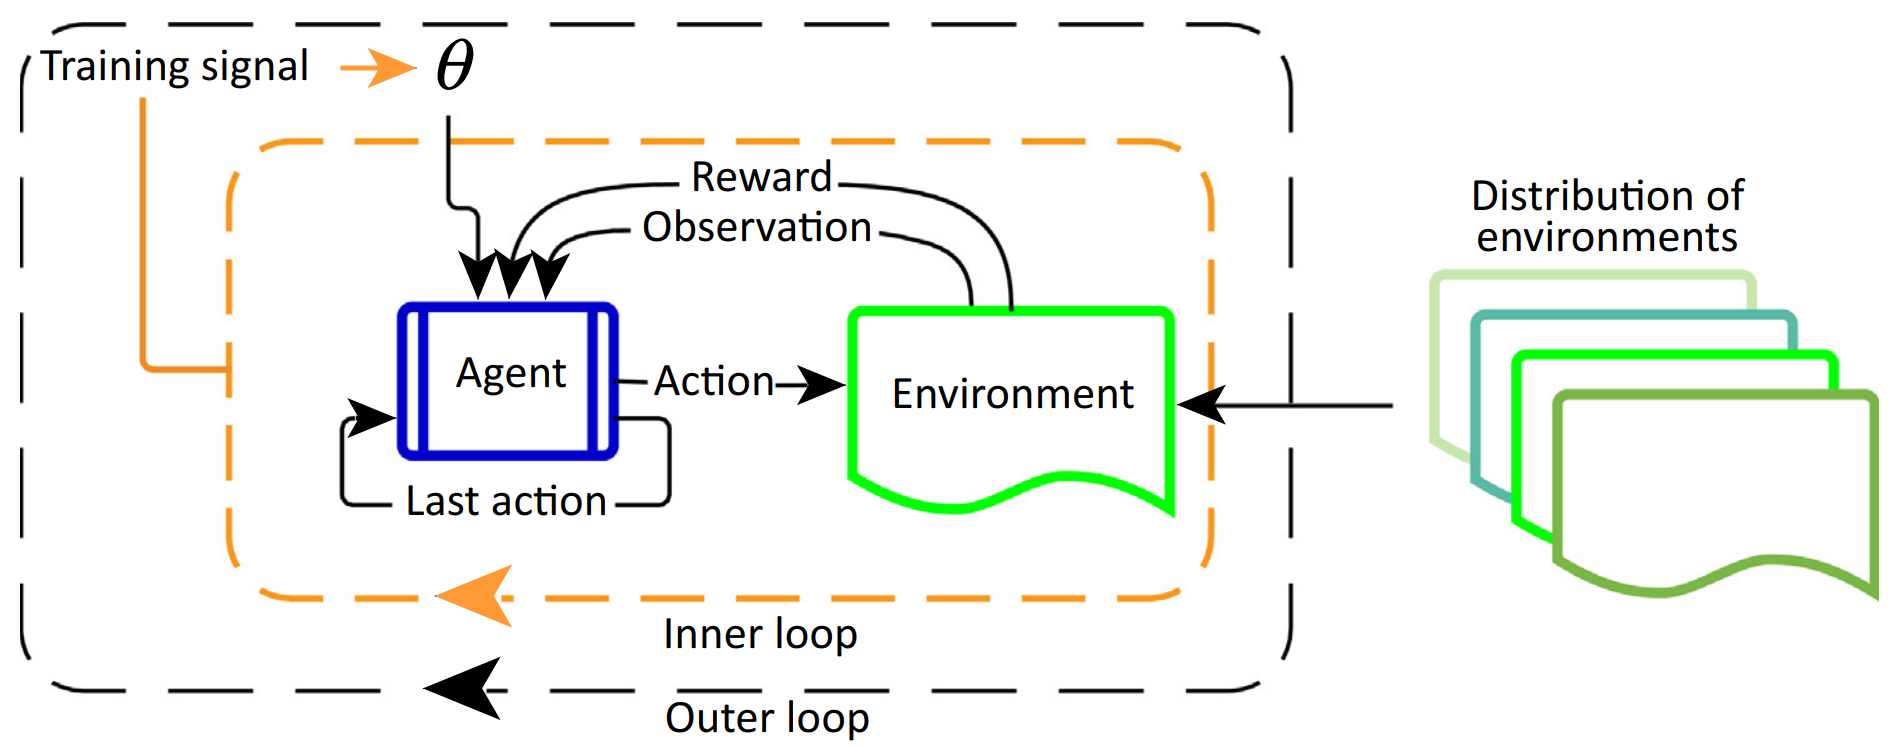
\includegraphics[scale=0.35]{meta-rl.png}
	\centering
	\caption{Schematic of meta-reinforcement Learning. The outer loop trains the parameter weights $\theta$, which determine the inner-loop learner ("Agent", instantiated by a recurrent neural network) that interacts with an environment for the duration of the episode. For every cycle of the outer loop, a new environment is sampled from a distribution of environments, which share some common structure.\cite{meta-model}}
	\label{meta-model}
\end{figure}

The agent is trained over specific learning tasks and optimized for the best performance in the inner loop, while in outer loop, the parameter of the learner is adjusted accordingly to yield the best performance on a distribution of tasks, including potentially unseen tasks.